\scanpage{50}
\mspage{4}
\figure{
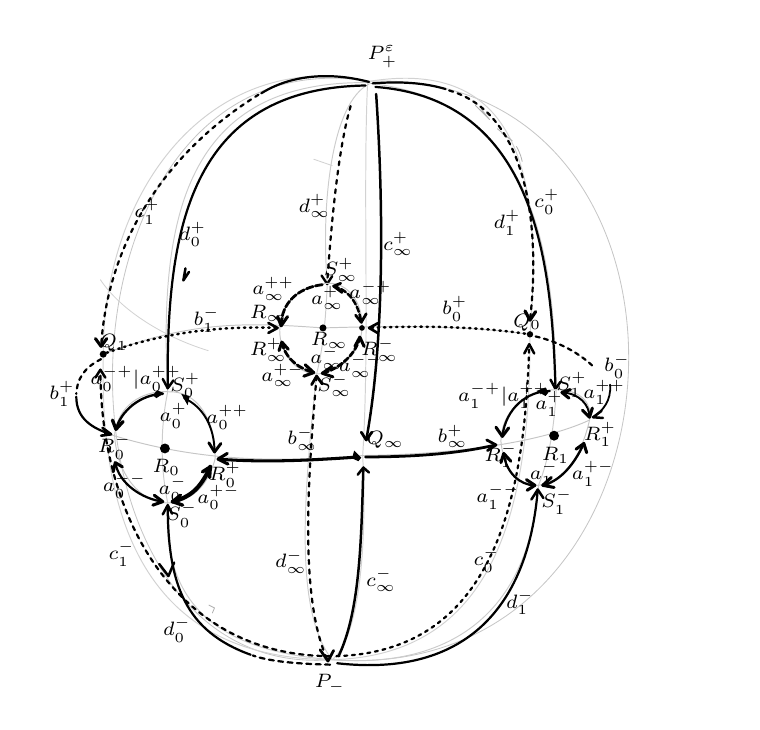
\begin{tikzpicture}[x=.009cm,y=-.009cm,>=stealth,every node/.style={font=\scriptsize},line cap=round,line join=round]
\draw[gray!45,line width=.3pt] (530,200) .. controls (63,125) and (48,1050) .. (477,1016) .. controls (1010,1055) and (1040,180) .. (530,200);
\draw[gray!35,line width=.35pt] (530,200) .. controls (310,152) and (154,347) .. (154,585) .. controls (147,879) and (256,1015) .. (477,1016);
\draw[gray!35,line width=.35pt] (530,200) .. controls (738,167) and (775,330) .. (756,557) .. controls (757,813) and (702,1010) .. (477,1016);
\draw[gray!35,line width=.35pt] (527,201) .. controls (520,349) and (530,575) .. (520,728) .. controls (527,866) and (513,988) .. (477,1016);
\draw[gray!40,line width=.35pt] (530,202) .. controls (269,197) and (232,394) .. (245,638) .. controls (234,691) and (235,747) .. (245,795) .. controls (235,951) and (333,1005) .. (477,1016);
\draw[gray!40,line width=.35pt] (530,203) .. controls (768,229) and (790,453) .. (793,635) .. controls (791,677) and (785,728) .. (768,770) .. controls (753,963) and (630,1028) .. (477,1016);
\draw[gray!40,line width=.35pt] (529,204) .. controls (476,230) and (461,374) .. (470,485) .. controls (468,537) and (464,577) .. (455,613) .. controls (436,791) and (424,949) .. (477,1016);
\draw[gray!45,line width=.35pt] (154,585) .. controls (278,538) and (355,540) .. (464,548) .. controls (591,544) and (671,546) .. (756,557);
\draw[gray!45,line width=.35pt] (166,699) .. controls (280,734) and (386,739) .. (520,728) .. controls (670,726) and (779,706) .. (840,678);
\draw[gray!35,line width=.3pt] (150,480) .. controls (178,522) and (237,560) .. (302,580);
\draw[gray!35,line width=.3pt] (451,310) -- (477,319);
\draw[gray!60,line width=.3pt] (679,234)--(699,254)--(687,239) (710,267)--(731,284)--(716,273) (737,292) .. controls (743,303) and (744,309) .. (745,313);
\draw[gray!60,line width=.3pt] (303,939)--(311,943)--(308,950);
\draw[line width=.8pt] (529,201) .. controls (476,187) and (420,190) .. (377,217);\draw[line width=.8pt,dash pattern=on 1.4pt off 1.8pt] (373,219) .. controls (239,302) and (160,430) .. (151,574);\draw[line width=1.1pt] (143,563)--(151,574)--(159,563);
\draw[line width=.8pt,dash pattern=on 1.6pt off 1.7pt] (475,1011) .. controls (260,1011) and (150,820) .. (150,607);\draw[line width=.9pt] (143,618)--(150,607)--(157,618);
\draw[line width=.8pt] (534,203) .. controls (572,200) and (607,202) .. (637,211);\draw[line width=.8pt,dash pattern=on 1.5pt off 1.7pt] (642,213) .. controls (754,245) and (771,409) .. (756,537);\draw[line width=1.15pt] (749,524)--(756,537)--(764,525);
\draw[line width=.8pt,dash pattern=on 1.1pt off 1.7pt] (483,1011) .. controls (708,1004) and (749,784) .. (755,571);\draw[line width=.9pt] (748,584)--(755,571)--(762,584);
\draw[line width=.9pt] (539,218) .. controls (550,382) and (550,572) .. (525,706);\draw[line width=1pt] (518,695)--(525,706)--(533,695);
\draw[line width=.9pt] (486,1011) .. controls (517,946) and (518,842) .. (521,745);\draw[line width=.9pt] (513,755)--(521,745)--(529,752);
\draw[line width=.8pt] (524,206) .. controls (273,210) and (243,415) .. (245,633);\draw[line width=.9pt] (270,464)--(267,481)--(275,469) (238,620)--(245,633)--(253,622);
\draw[line width=.8pt] (538,208) .. controls (763,225) and (787,453) .. (792,634);\draw[line width=.9pt] (785,621)--(792,634)--(799,624);
\draw[line width=.8pt,dash pattern=on 1.4pt off 2pt] (503,235) .. controls (486,293) and (476,396) .. (470,484);\draw[line width=.85pt] (462,474)--(470,486)--(477,475);
\draw[line width=.8pt,dash pattern=on 1.8pt off 1.6pt] (474,1023) .. controls (432,1022) and (390,1019) .. (365,1010);\draw[line width=.8pt] (362,1009) .. controls (270,976) and (245,910) .. (245,798);\draw[line width=.9pt] (238,811)--(245,798)--(251,810) (233,881)--(246,898)--(254,879);
\draw[line width=.8pt] (484,1021) .. controls (670,1042) and (754,936) .. (767,776);\draw[line width=.9pt] (758,790)--(767,776)--(775,788);
\draw[line width=.8pt,dash pattern=on 1.5pt off 2pt] (455,616) .. controls (443,758) and (430,930) .. (471,1018);\draw[line width=1pt] (448,628)--(455,616)--(463,627) (460,1002)--(471,1018)--(479,1003);
\draw[line width=.9pt,dash pattern=on .5pt off 1.7pt] (159,583) .. controls (245,552) and (329,545) .. (400,548);\draw[line width=.95pt] (387,541)--(400,548)--(387,555);
\draw[line width=.9pt,dash pattern=on .5pt off 1.7pt] (749,556) .. controls (673,545) and (593,545) .. (529,548);\draw[line width=.95pt] (542,541)--(529,548)--(541,555);
\draw[line width=1.1pt] (514,730) .. controls (445,735) and (379,738) .. (316,733);\draw[line width=1.1pt] (329,725)--(316,733)--(330,740);\fill (508,721)--(518,731)--(514,736)--(505,732)--cycle;
\draw[line width=1pt] (524,730) .. controls (594,730) and (656,725) .. (708,713);\draw[line width=1pt] (695,706)--(708,713)--(696,721);
\draw[line width=.8pt,dash pattern=on 1.5pt off 1.7pt] (151,592) .. controls (125,605) and (117,622) .. (116,641);\draw[line width=.8pt] (116,645) .. controls (116,677) and (140,690) .. (165,698);\draw[line width=.95pt] (153,689)--(165,698)--(151,700);
\draw[line width=.8pt,dash pattern=on 1.5pt off 1.6pt] (764,560) .. controls (803,569) and (831,588) .. (848,605);\draw[line width=.65pt] (869,628) .. controls (871,650) and (859,665) .. (845,674);\draw[line width=.9pt] (857,665)--(845,674)--(859,675);
\draw[gray!45,line width=.35pt] (245,638) .. controls (287,636) and (312,677) .. (312,732) .. controls (301,775) and (275,793) .. (245,795) .. controls (204,794) and (173,752) .. (170,699) .. controls (174,658) and (209,636) .. (245,638);
\draw[line width=.85pt] (238,641) .. controls (206,642) and (179,665) .. (172,691);\draw[line width=1.2pt] (167,678)--(172,691)--(182,680);\fill (230,636)--(240,640)--(229,647)--(224,643)--cycle;
\draw[line width=.7pt] (268,647) .. controls (295,659) and (311,688) .. (311,723);\draw[line width=1.05pt] (303,710)--(311,723)--(320,711);\fill (264,641)--(276,644)--(273,657)--cycle;
\draw[line width=.8pt] (171,738) .. controls (176,767) and (208,789) .. (238,793);\draw[line width=1.1pt] (168,751)--(171,738)--(181,744) (226,784)--(238,793)--(224,798);
\draw[line width=1.5pt] (305,744) .. controls (291,775) and (276,787) .. (252,793);\draw[line width=1.25pt] (294,751)--(305,744)--(304,759) (263,784)--(252,793)--(266,798);
\draw[gray!45,line width=.35pt] (793,635) .. controls (828,635) and (845,655) .. (840,678) .. controls (829,727) and (805,765) .. (768,770) .. controls (736,771) and (718,741) .. (715,708) .. controls (715,666) and (750,636) .. (793,635);
\draw[line width=.8pt] (784,637) .. controls (752,637) and (722,661) .. (717,701);\draw[line width=1.1pt] (708,688)--(717,701)--(726,689);\fill (778,632)--(765,637)--(778,644)--(782,639)--cycle;
\draw[line width=.7pt] (801,639) .. controls (826,640) and (840,657) .. (840,674);\draw[line width=1.1pt] (813,635)--(801,639)--(811,647) (830,664)--(840,674)--(844,661);
\draw[line width=.8pt] (719,725) .. controls (722,752) and (742,770) .. (763,770);\draw[line width=1.1pt] (715,738)--(719,725)--(729,736) (751,762)--(763,770)--(752,777);
\draw[line width=.85pt] (832,711) .. controls (817,744) and (796,765) .. (774,770);\draw[line width=1.1pt] (821,719)--(832,711)--(836,724) (786,759)--(774,770)--(790,773);
\draw[gray!45,line width=.35pt] (470,485) .. controls (500,483) and (521,514) .. (519,548) .. controls (518,586) and (483,612) .. (455,613) .. controls (424,611) and (403,583) .. (403,552) .. controls (402,518) and (430,487) .. (470,485);
\draw[line width=1pt,dash pattern=on 2.5pt off .9pt] (463,487) .. controls (429,491) and (405,513) .. (405,545);\draw[line width=1.1pt] (400,532)--(405,545)--(414,532);
\draw[line width=.9pt,dash pattern=on 2pt off .9pt] (479,489) .. controls (505,496) and (515,520) .. (518,540);\draw[line width=1pt] (489,485)--(479,489)--(491,498) (510,530)--(518,540)--(525,528);
\draw[line width=1pt,dash pattern=on 2.4pt off 1pt] (406,568) .. controls (411,593) and (434,607) .. (451,611);\draw[line width=1.1pt] (402,580)--(406,568)--(415,578) (439,600)--(451,611)--(437,616);
\draw[line width=1pt,dash pattern=on 2pt off .9pt] (516,561) .. controls (510,588) and (483,607) .. (463,612);\draw[line width=1.1pt] (509,574)--(516,561)--(522,574) (476,603)--(463,612)--(478,617);
\fill (154,585) circle (1.27pt);
\fill (756,557) circle (1.15pt);
\fill (241,718) circle (1.79pt);
\fill (790,700) circle (1.79pt);
\fill (464,548) circle (1.27pt);
\fill (519,548) circle (1.02pt);
\node at (548,165) {$P_+^{\deleted{\unsure{\varepsilon}}}$};
\node at (474,1050) {$P_-$};
\node at (169,569) {$Q_1$};
\node at (752,540) {$Q_0$};
\node at (552,706) {$Q_\infty$};
\node at (243,745) {$R_0$};
\node at (792,728) {$R_1$};
\node at (473,566) {$R_\infty$};
\node at (170,716) {$R_0^-$};
\node at (326,755) {$R_0^+$};
\node at (715,728) {$R_1^-$};
\node at (855,698) {$R_1^+$};
\node at (387,579) {$R_\infty^+$};
\node at (544,579) {$R_\infty^-$};
\node at (270,629) {$S_0^+$};
\node at (265,812) {$S_0^-$};
\node at (815,628) {$S_1^+$};
\node at (794,793) {$S_1^-$};
\node at (489,466) {$S_\infty^+$};
\node at (480,629) {$S_\infty^-$};
\node at (216,384) {$c_1^+$};
\node at (180,867) {$c_1^-$};
\node at (780,370) {$c_0^+$};
\node at (695,875) {$c_0^-$};
\node at (570,430) {$c_\infty^+$};
\node at (546,904) {$c_\infty^-$};
\node at (280,416) {$d_0^+$};
\node at (258,974) {$d_0^-$};
\node at (724,400) {$d_1^+$};
\node at (742,935) {$d_1^-$};
\node at (452,376) {$d_\infty^+$};
\node at (419,878) {$d_\infty^-$};
\node at (300,537) {$b_1^-$};
\node at (650,521) {$b_0^+$};
\node at (435,704) {$b_\infty^-$};
\node at (647,701) {$b_\infty^+$};
\node at (96,641) {$b_1^+$};
\node at (879,602) {$b_0^-$};
\node at (200,620) {$\unsure{a_0^{-+}|a_0^{++}}$};
\node at (329,674) {$a_0^{++}$};
\node at (184,771) {$a_0^{--}$};
\node at (317,787) {$\unsure{a_0^{+-}}$};
\node at (253,672) {$a_0^+$};
\node at (252,775) {$a_0^-$};
\node at (719,644) {$\unsure{a_1^{-+}|a_1^{++}}$};
\node at (861,639) {$a_1^{++}$};
\node at (711,786) {$\unsure{a_1^{--}}$};
\node at (845,754) {$\unsure{a_1^{+-}}$};
\node at (783,655) {$a_1^+$};
\node at (776,753) {$a_1^-$};
\node at (394,493) {$a_\infty^{++}$};
\node at (531,498) {$\unsure{a_\infty^{-+}}$};
\node at (407,615) {$\unsure{a_\infty^{+-}}$};
\node at (517,601) {$a_\infty^{--}$};
\node at (470,506) {$a_\infty^+$};
\node at (469,590) {$a_\infty^-$};
\node at (387,528) {$\deleted{\unsure{R_\infty}}$};
\end{tikzpicture}
}
On introduit
\[
(16)\quad\left\{\begin{array}{l}
Q_i\ (i\in J)^{\unsure{*}}\text{ antipodique de }R_i\ \inserted{(=-R_i)}\\
R_i^\omega\in U_i\quad(i\in J,\omega\in\uline{\omega})\\
P_\varepsilon\ \deleted{\unsure{\in}}\quad(\varepsilon\in\uline{\varepsilon}=\Pi_0(\Sigma\setminus\Sigma_{\mathbb R})\\
S_i^{\unsure{\varepsilon}}
\end{array}\right.
\]
où $P_\varepsilon$ est défini par
\[
(17)\qquad\{P_\varepsilon\}=\Delta\cap\unsure{(|\{}\Sigma-\Sigma_{\mathbb R})_\varepsilon
\]
\deleted{\unsure{des} $R_i^\omega\in U_{i\mathbb R}\unsure{\simeq\omega}$}
et $R_{i\omega}$ est défini ainsi

On a une bijection canonique
\[
(18)\qquad U_{i\mathbb R}\overset{\mathrm{def}}=\underbrace{U_i\cap T_{\Sigma_{\mathbb R},R_i}}_{TU_{\Sigma_{\mathbb R},R_i}}\simeq\omega
\]
sur \unsure{cette} variété \inserted{$\Sigma_{\mathbb R}$} de dim 1, l'une des orientations de celle-ci en les \unsure{points|point} $R_i$ (donc globalement) est en corr biunivoque avec l'une des deux directions orientées tangentes.
\margin{
\[
(19)\quad S_i^\varepsilon\in U_i\cap T_{\Sigma_i}\unsure{,}=TU_{\Sigma_i}\ \deleted{\unsure{de}}
\]
\deleted{\illegible{1} \unsure{qui}}
où $\Sigma_i$ est le grand cercle déterminé par les $P_\varepsilon^{\deleted{\unsure{\omega}}}$ et $Q_i$ on a $TU_{\Sigma_i}\simeq\uline{\varepsilon}$
Car les deux directions tangentes à $\Sigma_i$ en $R_i$ se distinguent suivant les deux hémisphères $\in\uline{\varepsilon}=\Pi_0(\Sigma\setminus\Sigma_{\mathbb R})$
}
\margin{\uline{NB} Il faudrait introduire $\widetilde\Sigma_{\deleted{\unsure{\varepsilon}}}^{(\varepsilon)}$ $(\varepsilon\in\uline{\varepsilon})$, les deux hémisphères sur $\widetilde\Sigma$, le choix des $S_i^\varepsilon$ est caractérisé par $S_i^\varepsilon\in\widetilde\Sigma_{\deleted{\unsure{\varepsilon}}}^{(\varepsilon)}$}
On a fait la figure en indexant
\[
J=\{0,1,\infty\}\qquad \uline{\omega}=\{+1,-1\}
\]
et en choisissant une orientation sur le sphère, i.e
\[
\uline{\unsure{\omega}}\simeq\{+1,-1\},\quad\text{d'où }\varepsilon\simeq\{+1,-1\}.
\]
\margin{$+$ donné par la perm. circulaire $1\to2\to3$\quad $-$ par l'inverse}
\deleted{On définit des \unsure{arcs de cercle} sur $\widetilde\Sigma$}
\deleted{\inserted{choisit des chemins}}
\deleted{\unsure{liant} des points de $\widetilde\Sigma$}
\deleted{$(19)\qquad a_i^\omega,\ b_i,\ c_i^\omega$}
\deleted{On choisit dorénavant une orientation de $\unsure{\Sigma}$}
\deleted{(pour \unsure{introduire|intérieurs} des}
\deleted{(pour les $b_i^\omega$)}
\deleted{\unsure{notations pléthoriques} \illegible{1}}
\margin{49}
